\section{CTL Commands}

\subsection{ctl}
Das Hauptkommando. Hierüber besteht Zugriff auf alle anderen Befehle wie
\emph{git} es tun würde :-).

So kann z.B. das Kommando
\subsection{ctl-genmanifest}
\subsection{ctl-web}
\subsection{ctl-init}
\subsection{ctl-runcgi}
\subsection{ctl-register}

\section{Entwürfe}

\subsection[Datenbank}
\begin{figure}[h]
\centering
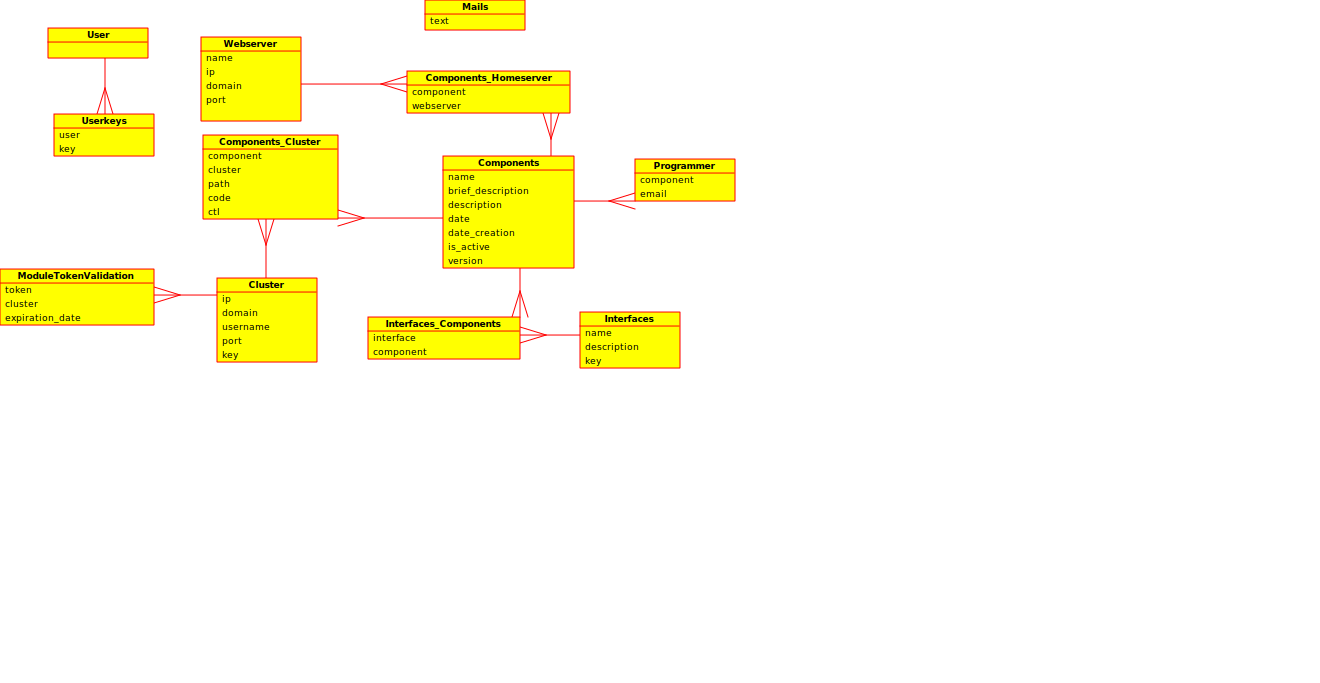
\includegraphics[width=0.8\linewidth]{Bilder/ctl-db.svg}
\caption[CTL-DB]{CTL-DB}
\label{CTL-Datenbank}
\end{figure}
